\Problem{Sliding Cube in a Bowl}{\SliCuBowl}{
A small cube of mass $ m $ slides back and forth in a frictionless, hemispherical bowl of radius $ R $. Suppose the cube is released at angle $ \theta $. What is the cube's speed at the bottom of the bowl?
}
\ProblemFig{\SliCuBowlFig}{
\centering
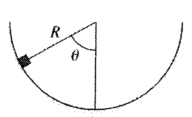
\includegraphics{\FileDepth/Activities/Sliding_Cube_in_a_Bowl/Bowl_with_Cube_Setup.pdf}
}
\ProblemSub{\SliCuBowlA}{
(a) Begin by drawing a before-and-after pictorial representation. Let the cube's initial position and speed be $ y_{i} $ and $ v_{i} $. Use a similar notation for the final position and speed.
}
\Solution{\SliCuBowlASol}{
\begin{figure}[h]
	\centering
	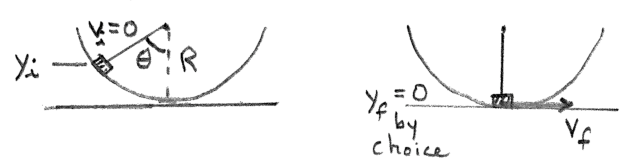
\includegraphics{\FileDepth/Activities/Sliding_Cube_in_a_Bowl/Bowl_with_Cube_Initial_and_Final.pdf}
\end{figure}
}
\ProblemSub{\SliCuBowlB}{
(b) At the initial position, are either $ K_{i} $ or $ U_{Gi} $ zero? If so, which?
}
\Solution{\SliCuBowlBSol}{

The cube is released from rest at the initial position, so $ K_{i} = 0 $ J.
}
\ProblemSub{\SliCuBowlC}{
(c) At the final position, are either $ K_{f} $ or $ U_{Gf} $ zero? If so, which?
}
\Solution{\SliCuBowlCSol}{

We can choose the zero of gravitational potential energy to be at the bottom of the bowl, so $ U_{Gf} = 0 $ J.
}
\ProblemSub{\SliCuBowlD}{
(d) Does thermal energy need to be considered in this situation? Why or why not?
}
\Solution{\SliCuBowlDSol}{

No, because the bowl is frictionless. There are no dissipative forces stealing energy from the system.
}
\ProblemSub{\SliCuBowlE}{
(e) Write the conservation of energy equation in terms of position and speed variables, omitting any terms that are zero.
}
\Solution{\SliCuBowlESol}{
\[
\begin{split}
	\cancel{K_{i}} + U_{Gi} & = K_{f} + \cancel{U_{Gf}} \\
	mgy_{i} & = \frac{1}{2}mv_{f}^{2}
\end{split}
\]
}
\ProblemSub{\SliCuBowlF}{
(f) You're given not the initial position but the initial angle. Do the geometry and trigonometry to find $ y_{i} $ in terms of $ R $ and $ \theta $.
}
\Solution{\SliCuBowlFSol}{
\begin{figure}[h]
	\centering
	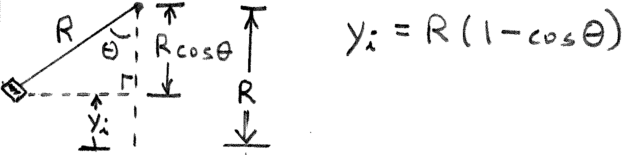
\includegraphics{\FileDepth/Activities/Sliding_Cube_in_a_Bowl/Bowl_with_Cube_Trig_Supplement.pdf}
\end{figure}
}
\ProblemSub{\SliCuBowlG}{
(g) Use your result of part (f) in the energy conservation equation, and then finish solving the problem.
}
\Solution{\SliCuBowlGSol}{
\[
\begin{split}
	mgy_{i} & = \frac{1}{2}mv_{f}^{2} \\
	\cancel{m}gR(1-\cos\theta) & = \frac{1}{2}\cancel{m}v_{f}^{2} \\
	\implies v_{f} & = \sqrt{2gR(1-\cos\theta)}
\end{split}
\]
}